% Created 2024-04-11 Thu 13:40
% Intended LaTeX compiler: xelatex
\documentclass[11pt]{article}
\usepackage{hyperref}
% TIPS
% \substack{a\\b} for multiple lines text





% pdfplots will load xolor automatically without option
\usepackage[dvipsnames]{xcolor}

\usepackage{forest}
% two-line text in node by [two \\ lines]
% \begin{forest} qtree, [..] \end{forest}
\forestset{
  qtree/.style={
    baseline,
    for tree={
      parent anchor=south,
      child anchor=north,
      align=center,
      inner sep=1pt,
    }}}
%\usepackage{flexisym}
% load order of mathtools and mathabx, otherwise conflict overbrace

\usepackage{mathtools}
%\usepackage{fourier}
\usepackage{pgfplots}
\usepackage{amsthm, mathabx,  amsmath, commath}
\usepackage{amsfonts}

\usepackage{empheq}
\usepackage{tikz}
\usetikzlibrary{arrows.meta}
\usepackage[most]{tcolorbox}

\newtheorem{theorem}{Theorem}[section]
\newtheorem{definition}{Definition}[section]
\newtheorem{corollary}{Corollary}[section]
\newtheorem{example}{Example}[section]
\newtheorem{lemma}{Lemma}[section]
\newtheorem{proposition}{Proposition}[section]

\newcommand{\bl}[1] {\boldsymbol{#1}}
\newcommand{\Wt}[1] {\stackrel{\sim}{\smash{#1}\rule{0pt}{1.1ex}}}
\newcommand{\wt}[1] {\widetilde{#1}}


%For boxed texts in align, use Aboxed{}
%otherwise use boxed{}

\DeclareMathSymbol{\widehatsym}{\mathord}{largesymbols}{"62}
\newcommand\lowerwidehatsym{%
  \text{\smash{\raisebox{-1.3ex}{%
    $\widehatsym$}}}}
\newcommand\fixwidehat[1]{%
  \mathchoice
    {\accentset{\displaystyle\lowerwidehatsym}{#1}}
    {\accentset{\textstyle\lowerwidehatsym}{#1}}
    {\accentset{\scriptstyle\lowerwidehatsym}{#1}}
    {\accentset{\scriptscriptstyle\lowerwidehatsym}{#1}}
}

\usepackage{graphicx}
    
% text on arrow for xRightarrow
\makeatletter
%\newcommand{\xRightarrow}[2][]{\ext@arrow 0359\Rightarrowfill@{#1}{#2}}
\makeatother


\def \bx {\boldsymbol{x}}
\def \ba {\boldsymbol{a}}
\def \bI {\boldsymbol{I}}
\def \bt {\boldsymbol{t}}
\def \bb {\boldsymbol{b}}
\def \bA {\boldsymbol{A}}
\def \bX {\boldsymbol{X}}
\def \bu {\boldsymbol{u}}
\def \bS {\boldsymbol{S}}
\def \bZ {\boldsymbol{Z}}
\def \bz {\boldsymbol{z}}
\def \by {\boldsymbol{y}}
\def \bw {\boldsymbol{w}}
\def \bT {\boldsymbol{T}}
\def \bS {\boldsymbol{S}}
\def \bm {\boldsymbol{m}}
\def \bW {\boldsymbol{W}}
\def \bY {\boldsymbol{Y}}
\def \bH {\boldsymbol{H}}
\def \blambda {\boldsymbol{\lambda}}
\def \bPhi {\boldsymbol{\Phi}}
\def \btheta {\boldsymbol{\theta}}
\def \bmu {\boldsymbol{\mu}}
\def \bphi {\boldsymbol{\phi}}
\def \bSigma {\boldsymbol{\Sigma}}
\def \lb {\left\{}
\def \rb {\right\}}
\def \caln {\mathcal{N}}
\def \dissum {\displaystyle\Sigma}
\def \dispro {\displaystyle\prod}
\def \E {\mathbb{E}}
\def \Q {\mathbb{Q}}
\def \V {\mathbb{V}}
\def \R {\mathbb{R}}
\def \calq {\mathcal{Q}}
\def \calg {\mathcal{G}}
\def \caln {\mathcal{N}}
\def \calr {\mathcal{R}}
\def \calm {\mathcal{M}}
\def \calc {\mathcal{C}}
\def \bcup {\bigcup}

\graphicspath{{../../books/}}
\makeindex

%% ox-latex features:
%   !announce-start, !guess-pollyglossia, !guess-babel, !guess-inputenc, caption,
%   underline, image, !announce-end.

\usepackage{capt-of}

\usepackage[normalem]{ulem}

\usepackage{graphicx}

%% end ox-latex features


\author{wu}
\date{\today}
\title{Db}
\hypersetup{
 pdfauthor={wu},
 pdftitle={Db},
 pdfkeywords={},
 pdfsubject={},
 pdfcreator={Emacs 29.1 (Org mode 9.7-pre)}, 
 pdflang={English}}
\begin{document}

\maketitle
\tableofcontents

\section{General}
\label{sec:org4df6460}
\subsection{Databases and Finite-Model Theory}
\label{sec:org648fcfc}
In a very real sense, finite-model theory provides the backbone of database theory. And databases
provide a concrete scenario for finite-model theory.

The overlap of database theory with nite-model theory occurs primarily in the area of query languages.

Shit paper
\section{Storage}
\label{sec:orgfc60dd4}
\subsection{LSM-based Storage Techniques: A Survey}
\label{sec:orgb4f8147}
\url{https://doi.org/10.1007/s00778-019-00555-y}
LSM-tree: bigtable, dynamo, hbase, cassandra, leveldb, rocksdb, asterixdb
\subsubsection{LSM-tree basics}
\label{sec:org34a5b2f}
\begin{enumerate}
\item Basic Structure
\label{sec:org9b88568}
\begin{itemize}
\item Memory component: concurrent data structure, skip-list/\(B^+\)-tree
\item Disk component, SSTables: a data block stores key-value pairs ordered by keys, and the index blocks
stores the key ranges of all data blocks
\end{itemize}

Two types of merge policies:
\begin{center}
\includegraphics[width=.8\textwidth]{../images/db/4.png}
\captionof{figure}{\label{}LSM-tree merge policies}
\end{center}
\begin{itemize}
\item \textbf{Leveling merge policy}: each level only maintains one component, but the component at level \(L\) is
\(T\) times larger than the component at level \(L-1\). As a result, the component at level \(L\)
will be merged multiple times with incoming component at level \(L-1\) until it fills up, and it
will then be merged into level \(L+1\), and it will then be merged into level \(L+1\).

\uline{Better query performance}.
\item \textbf{Tiering merge policy}: maintains up to \(T\) components per level. When level \(L\) is full, its
\(T\) components are merged together into a new component at level \(L+1\).

\uline{Better write performance}.
\end{itemize}
\item Well-Known Optimizations
\label{sec:org0198a08}
\textbf{Bloom filter}:
\begin{itemize}
\item built on top of disk components.
\item built for each leaf page for a disk component: a point lookup can first search the non-leaf pages of
a \(B^+\)-tree to locate the leaf page, where the non-leaf pages are assumed to be small enough to
be cached, and then check the associated Bloom filter before fetching the leaf page.
\end{itemize}
The false positive rate of a Bloom filter is
\begin{equation*}
\left(1-e^{-kn}/m\right)^k
\end{equation*}
where \(k\) is the number of hash functions, \(n\) is the number of keys, and \(m\) is the total
number of bits. And the optimal number of hash functions that minimizes the false positive rate is
\begin{equation*}
k=\frac{m}{n}\ln 2
\end{equation*}
In practice, most systems typically use 10 bits/key as a default configuration, which gives a 1\% false
positive rate.

\textbf{Partitioning}: Partitioning is orthogonal to merge policies, both leveling and tiering can be adapted
to supported partitioning. But only the partitioned leveling policy has been fully implemented.

In the partitioned leveling merge policy, pioneered by LevelDB, the disk component at each level is
range partitioned into multiple fixed-size SSTables, as in figure \ref{lsm.4}
\begin{center}
\includegraphics[width=.8\textwidth]{../images/db/5.png}
\captionof{figure}{\label{lsm.4}Partitioned leveling merge policy}
\end{center}
Each SSTable is labeled with its key range in the figure. To merge an SSTable from level \(L\) into
level \(L+1\), all of its overlapping SSTable at level \(L+1\) are selected, and these SSTables are
merged with it to produce new SSTables still at level \(L+1\). Different policies can be used to
select which SSTable to merge next at each level.

The partitioned optimization can also be applied to the tiering merge policy. However, one major issue
in doing so is that each level can contain multiple SSTables with overlapping key ranges. Two possible
schemes can be used to organize the SSTables at each level
\begin{enumerate}
\item \textbf{Vertical grouping}: groups SSTables with overlapping key ranges together so that the groups have
disjoint key ranges
\item \textbf{Horizontal grouping}: each logical disk component, which is range-partitioned into a set of
SSTables, serves as a group directly
\end{enumerate}

\begin{center}
\includegraphics[width=.8\textwidth]{../images/db/6.png}
\captionof{figure}{\label{}Partitioned tiering with vertical grouping}
\end{center}
During a merge operation, all of the SSTables in a group are merged together to produce the resulting
SSTables based on the key ranges of the overlapping groups at the next level, which are then added to
these overlapping groups.

\begin{center}
\includegraphics[width=.8\textwidth]{../images/db/7.png}
\captionof{figure}{\label{}Partitioned tiering with horizontal grouping}
\end{center}
Each level \(L\) further maintains an active group, which is also the first group, to receive new
SSTables merged from the previous level. A merge operation selects the SSTables with overlapping key
ranges from all of the groups at a level, and the resulting SSTables are added to the active group at
the next level.
\item Concurrency Control and Recovery
\label{sec:org3270d4e}
Depending on the transactional isolation requirement, today's LSM-tree implementations either use a
locking scheme or a multi-version scheme. A multi-version scheme works well with an LSM-tree since
obsolete can be \uline{garbage-collected} during merges.

Concurrent flush and merge operations, however, are unique to LSM-tree. These operations modify the
metadata of an LSM-tree, e.g., the list of active components. Thus, accesses to the component metadata
must be properly synchronized. To prevent a component in use from being deleted, each component can maintain a \uline{reference counter}.
Before accessing the components of an LSM-tree, a query can first obtain a snapshot of active
components and increment their in-use counters.

Since all writes are first appended into memory, write-ahead logging (WAL) can be performed to ensure
their durability. To simplify the recovery process, existing systems typically employ a \textbf{no-steal}
\textbf{buffer management policy}: a memory component can only be flushed when all active write transactions
have terminated. During recovery for an LSM-tree, the transaction log is replayed to redo all
successful transactions, but no undo is needed due to the no-steal policy.

Meanwhile, the list of active disk components must also be recovered in the event of a crash.
\begin{itemize}
\item For unpartitioned LSM-trees, this can be accomplished by \uline{adding a pair of timestamps of the stored
entries}.

This timestamp can be simply generated using local wall-clock time or a monotonic sequence number.
To reconstruct the component list, the recovery process can simply find all components with disjoint
timestamps. In the event that multiple components have overlapping timestamps, the component with
the largest timestamp range is chosen and the rest can simply be deleted since they will have been
merged to form the selected component.
\item For partitioned LSM-trees, a typical approach is to maintain a separate metadata log to store all
changes to the structural metadata, such as adding or deleting SSTables. The state of the LSM-tree
structure can then be reconstructed by replaying the metadata log during recovery.
\end{itemize}
\item Cost Analysis
\label{sec:org0c0253b}
The cost of writes and queries is measured by counting the number of disk I/Os per operation. This
analysis considers an unpartitioned LSM-tree and represents a worst-case cost.

Define
\begin{align*}
T&=\text{size ratio of a given LSM-tree}\\
L&=\text{levels of the LSM-tree}\\
B&=\text{number of entries that each data page can store, page size}\\
P&=\text{number of pages of a memory component}
\end{align*}

As a result, a memory component will contain at most \(B\cdot P\) entries., and level \(i\) will
contain at most \(T^{i+1}\cdot B\cdot P\) entries. Given \(N\) total entries, the largest level
contains approximately \(N\cdot\frac{T}{T+1}\). Thus the number of levels for \(N\) entries can be
approximated as \(L=\ceil{\log_T\left(\frac{N}{B\cdot P}\cdot\frac{T}{T+1}\right)}\)

The write cost, which is also referred to as \textbf{write amplification} in the literature, measures the
amortized I/O cost of inserting an entry into an LSM-tree. It should be noted that this cost measures
the overall I/O cost for this entry to be merged into the largest level since inserting an entry into
memory does not incur any disk I/O.
\begin{itemize}
\item For leveling, a component at each level will be merge \(T-1\) times until it fills up and is pushed
to the next level.
\item For tiering, multiple components at each level are merged only once and are pushed to the next level
directly.
\end{itemize}

Since each disk page contains \(B\) entries, the write cost for each entry will be
\(O(T\cdot\frac{L}{B})\) for leveling and \(O(\frac{L}{B})\) for tiering.
\end{enumerate}
\section{Fault Tolerance}
\label{sec:orgd3fd548}
\subsection{Chain Replication for Supporting High Throughput and Availability}
\label{sec:org2959d5b}
This paper is concerned with storage systems that sit somewhere between file systems and database systems.

\textbf{strong consistency guarantees}:
\begin{enumerate}
\item operations to query and update individual objects are executed in some sequential order
\item the effects of update operations are necessarily reflected in results returned by subsequent query
operations.
\end{enumerate}


\begin{center}
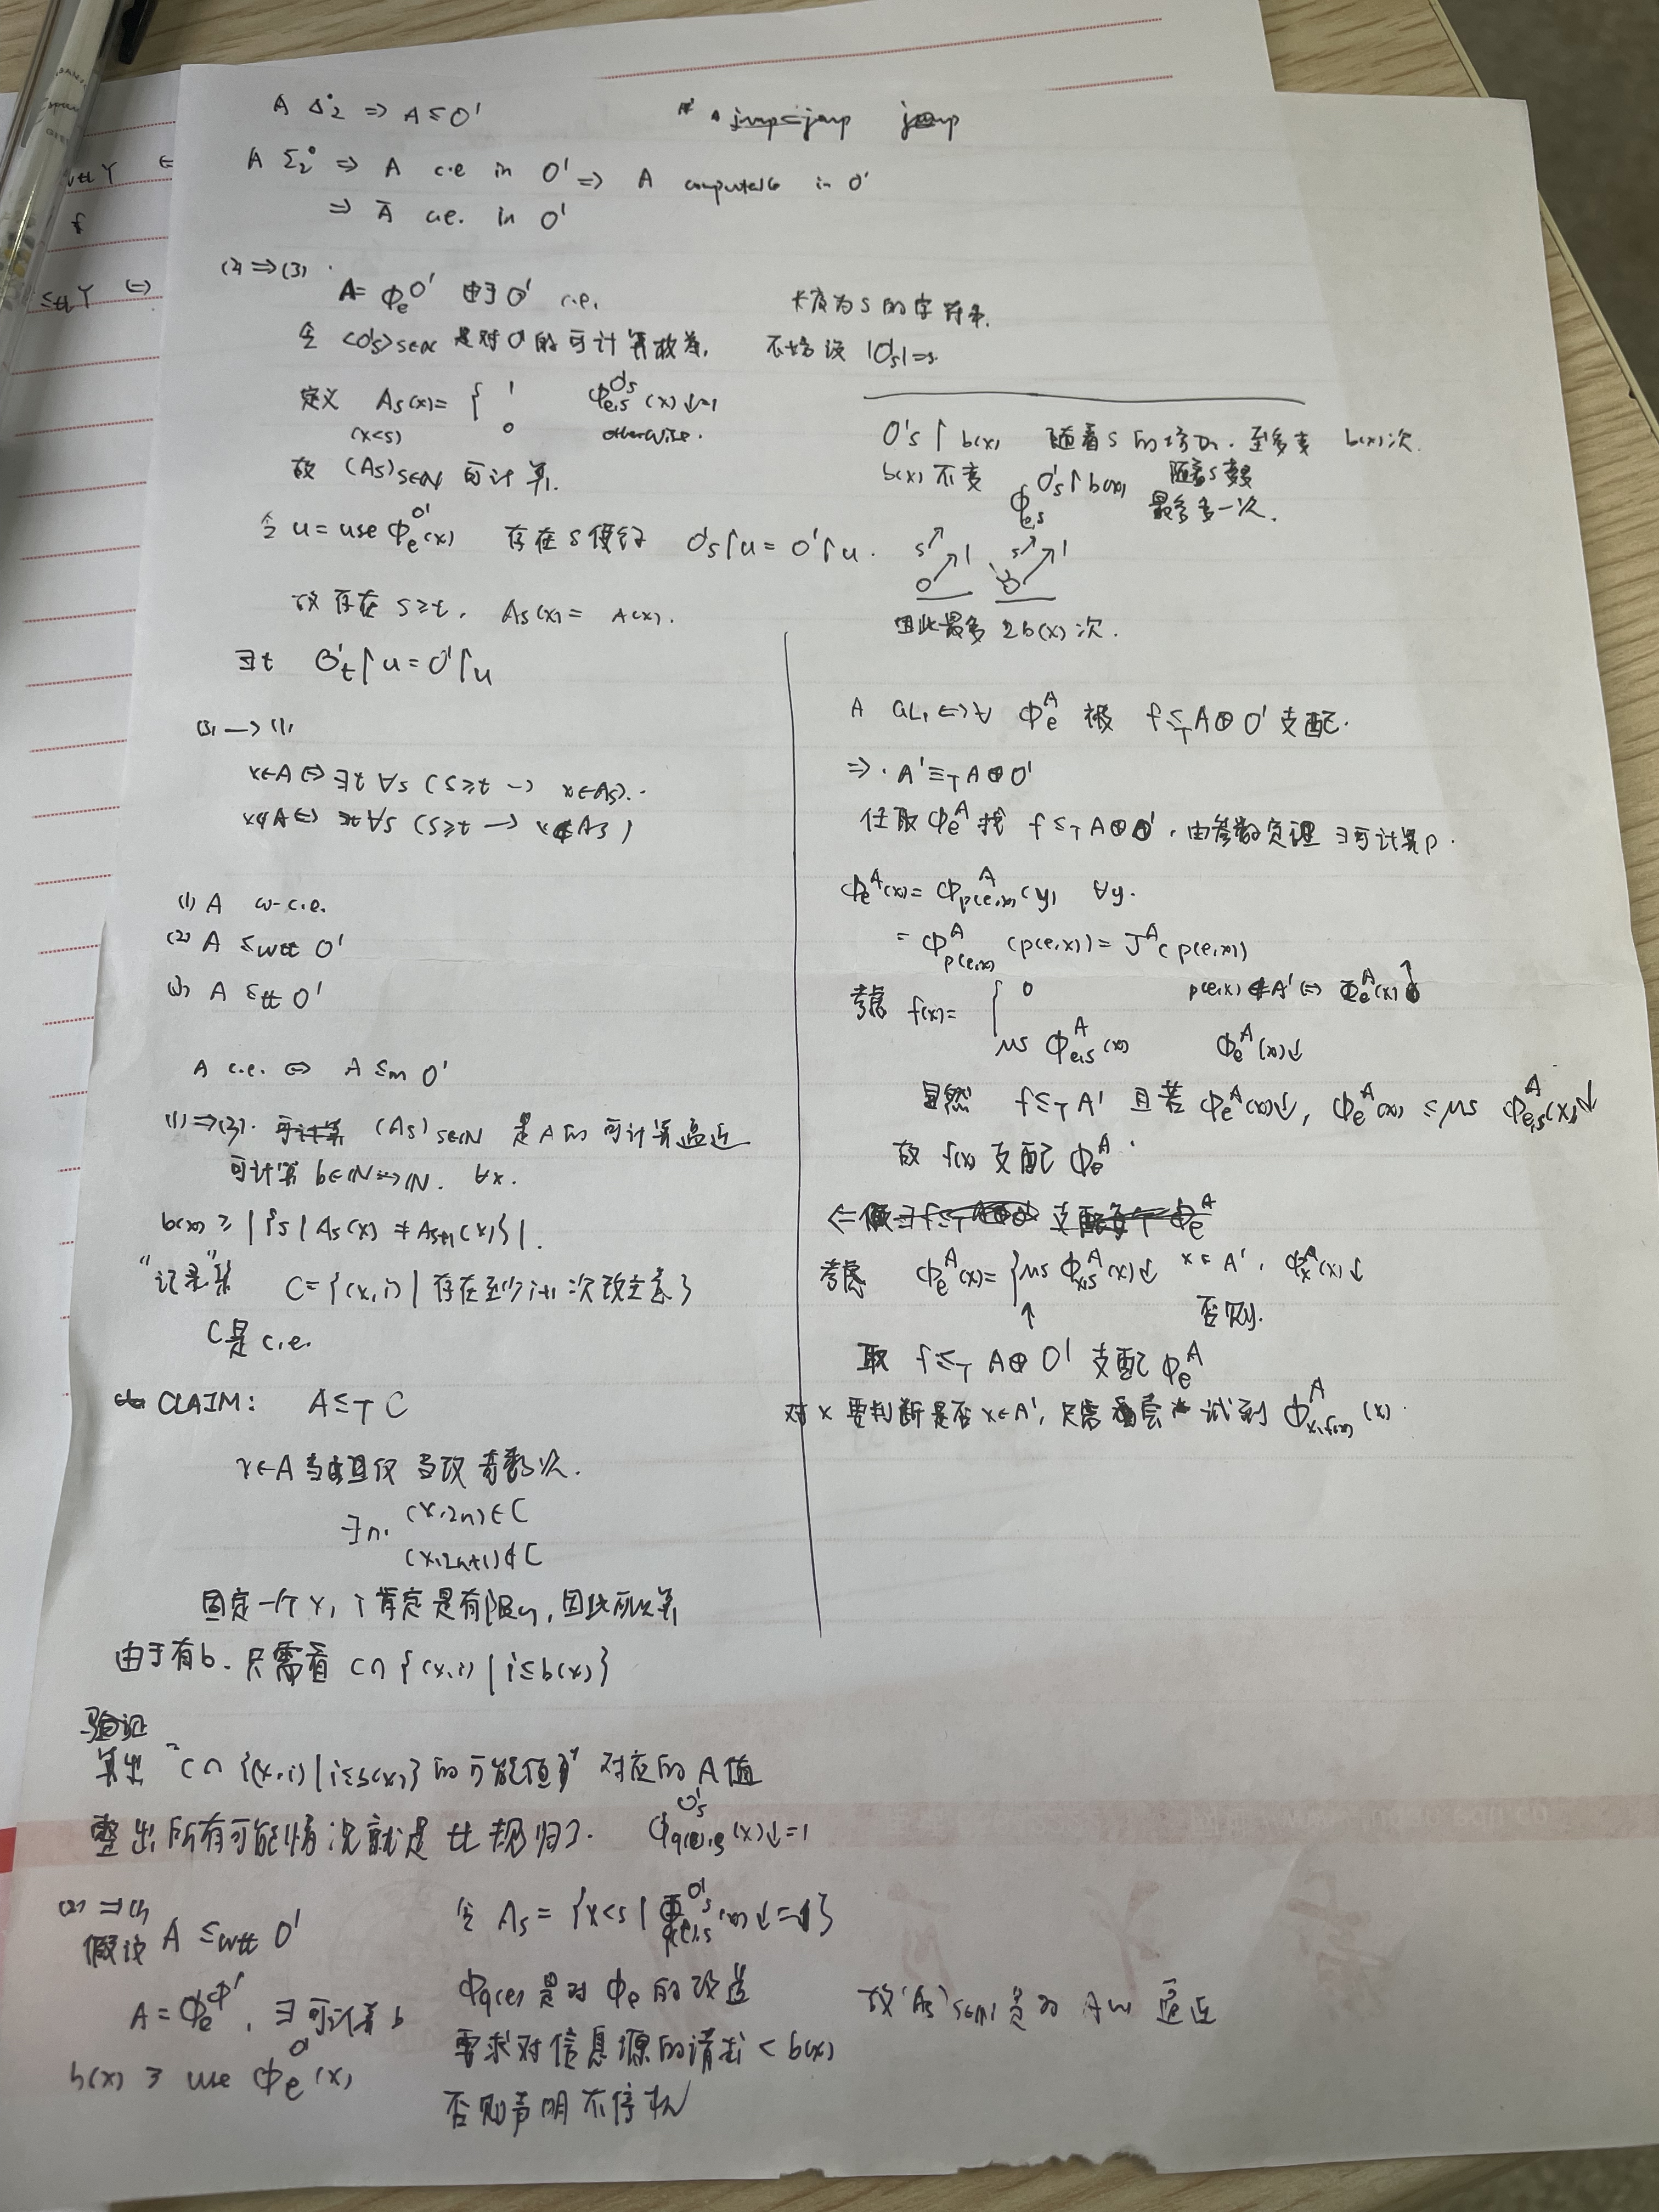
\includegraphics[width=.8\textwidth]{../images/db/1.png}
\captionof{figure}{\label{}Client's View of an Object}
\end{center}

Servers are assumed to be fail-stop:
\begin{enumerate}
\item each server halts in response to a failure rather than making erroneous state transitions, and
\item a server’s halted state can be detected by the environment.
\end{enumerate}


\begin{itemize}
\item \(Hist_{objID}\) is defined to be \(Hist_{objID}^T\), the value of \(Hist_{objID}\) stored by tail T of
the chain,
\item \(Pending_{objID}\) is defined to be the set of client requests received by any server in the chain and not yet processed by the tail.
\end{itemize}


\begin{enumerate}
\item a server in the chain receiving a request from a client
\item the tail processing a client request
\end{enumerate}


The master distinguishes three cases:
\begin{itemize}
\item failure of the head
\item failure of the tail
\item failure of some other server in the chain.
\end{itemize}


Let the server at the head of the chain be labeled \(H\), the next server be labeled \(H+1\), etc.,
through the tail, which is given label \(T\) . Define
\begin{equation*}
Hist_{objID}^i\preceq Hist^j_{objID}
\end{equation*}
to hold if sequence of requests \(Hist^i_{objID}\) at the server with label \(i\) is a prefix of
sequence \(Hist_{objID}^j\) at the server with label \(j\).

\textbf{Update Propagation Invariant}: For servers labeled \(i\) and \(j\) s.t. \(i\le j\) holds then
\begin{equation*}
Hist^j_{objID}\preceq Hist^i_{objID}
\end{equation*}
\textbf{Inprocess Requests Invariant}: If \(i\le j\) then
\begin{equation*}
Hist_{objID}^i=Hist^j_{objID}\oplus Sent_i
\end{equation*}
\end{document}
